%%%%%%%%%%%%%%%%%%%%%%%%%%%%%%%%%%%%%%%%%
% Introduction
%
% $Date$
% $Revision$
% $Author$


\chapter{Introduction}\label{chap:introduction}

Modern software applications are often complex and have to fulfill a large set of functional and non-functional properties. The internal behavior of such large systems cannot easily be determined on the basis of the source code. Furthermore, existing applications often lack sufficient documentation which makes it cumbersome to extend and change them for future needs. A solution to these problems can be monitoring, which allows to log the behavior of the application and to discover the application-internal control flows and response times of method executions.

The monitoring of the behavior can help in detecting performance problems and faulty behavior, capacity planning, and many other areas. The \Kieker{} framework provides the necessary monitoring capabilities and comes with tools and libraries for the analysis of monitored data. \Kieker{} was designed for %
continuous monitoring in production systems inducing only a very low overhead. A short overview on the overhead caused by \Kieker{} is provided at \url{https://se.informatik.uni-kiel.de/kieker/overhead-evaluation/}.
%, and offline evaluation of monitored data for a deeper inspection of the application's behavior and runtime architecture.

%%
\section{What is \Kieker?}\label{sec:kieker}

The present version of \Kieker{} is a monitoring and analysis framework for %
Java applications. %
Support for other platforms, such as .NET, is currently under development. %
Figure \ref{fig:KiekerComponentDiagram} shows the framework's composition based %
on the two main components \KiekerMonitoringPart{} and \KiekerAnalysisPart{}. %

% This is the component diagram of Kieker (the satellite).
\begin{figure}[H]\centering
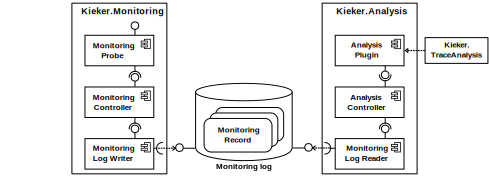
\includegraphics[width=0.98\textwidth]{images/kiekerComponentDiagram-woCloud-bw-w-record-newNames-withTraceAnalysis}
\caption{Overview of the framework components}
\label{fig:KiekerComponentDiagram}
\end{figure}
		
\noindent The \KiekerMonitoringPart{} component is responsible for program instrumentation, data collection, and logging. Its core is the \class{MonitoringController}. %  which %
%receives the monitoring data in so-called monitoring records from monitoring probes, and writes these %
% receives the monitoring data and passes it to the configured monitoring log writer. %
%
The component \KiekerAnalysisPart{} is responsible for reading, analyzing, and visualizing the monitoring data. Its core is the \class{AnalysisController} which manages the life-cycle of the monitoring reader and all analysis plugins.

The monitoring and analysis parts of the \Kieker{} framework are composed of subcomponents which represent the different functionalities of the monitoring and analysis tasks. The important interaction pattern among the components is illustrated in Figure~\ref{fig:KiekerCommunicationDiagram} but will be explained furthermore throughout the course of this user guide.

\vspace{1cm}

% This image shows the communication diagram of the different components.
\begin{figure}[H]\centering
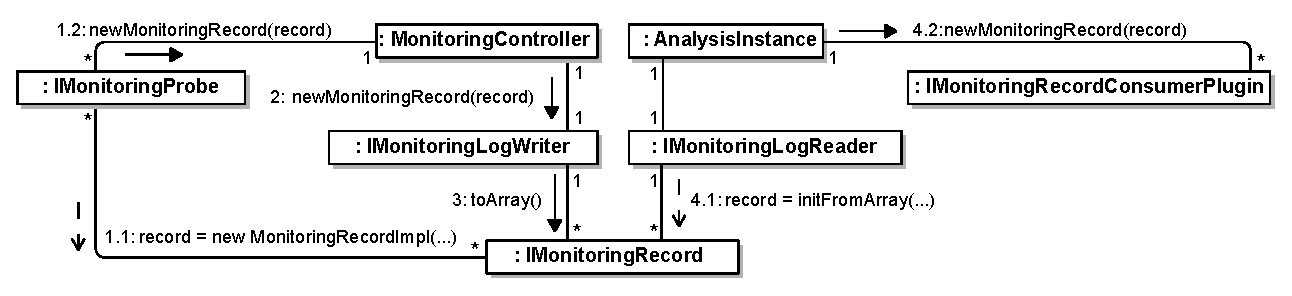
\includegraphics[width=1\textwidth]{images/kiekerCommunications-revisedReArranged-woMonitoringLog-bw-newNames}
\caption{Communication among \Kieker{} framework components}
\label{fig:KiekerCommunicationDiagram}
\end{figure}

\vspace{1cm}

% Notify-tag because it is explained how Kieker works.
% avh: removed
\noindent The monitoring probes create the monitoring records containing the %
monitoring data and deliver them to the monitoring controller. %
The monitoring controller employs the monitoring writers to write these %
monitoring records to a monitoring log or stream. %
For analyzing purposes, a monitoring reader reads the records from the monitoring log/stream. %
These records can then be further processed by the analysis plugins.

%%
% \section{Features}

Kieker includes monitoring writers and readers for filesystems, SQL %
databases, and the Java Messaging Service~(JMS)~\cite{JMS-WebSite}. %
A special feature of \Kieker{} is the ability to monitor and analyze (distributed) %
traces of method executions and corresponding timing information. %
For monitoring this data, Kieker includes monitoring probes employing %
AspectJ~\cite{AspectJ-WebSite}, %
Java~EE Servlet~\cite{JavaServletTechnology-WebSite}, %
Spring~\cite{Spring-WebSite}, and %
Apache~CXF~\cite{CXF-WebSite} technology. %
The \KiekerTraceAnalysis{} tool, itself implemented as a \KiekerAnalysisPart{} %
plugin (Figure~\ref{fig:KiekerComponentDiagram}), allows to reconstruct and visualize architectural models of the monitored %
systems, e.g., as sequence and dependency diagrams.

%%
\pagebreak

\section{Structure of this User Guide}

Based on a simple example, Chapter~\ref{chap:example} demonstrates %
how to manually instrument Java programs with \KiekerMonitoringPart{} %
in order to monitor timing information of method executions, and %
how to use \KiekerAnalysisPart{} to analyze the monitored data. %
Chapter~\ref{chap:componentsMonitoring} provides a more detailed %
description of \KiekerMonitoringPart{} and shows how to implement and %
use custom monitoring records, monitoring probes, and monitoring writers. %
A more detailed description of \KiekerAnalysisPart{} and how to implement and use %
custom monitoring readers, and analysis plugins follows in %
Chapter~\ref{chap:componentsAnalysis}. %
Chapter~\ref{chap:aspectJ} demonstrates how to use \KiekerTraceAnalysis{} %
for monitoring, analyzing, and visualizing trace information. %
Additional resources are included in the appendix.

\quad\\

% Notify-tag because this could be interesting for the reader.
\NOTIFYBOX{The Java sources presented in this user guide are included in the %
\file{\exampleDir/} directory of the \Kieker{} distribution (see %
Section~\ref{sec:example:downloadInstall}).}


% \TODO{Point to Web site for additional examples, TR, \ldots}
